\documentclass{article}

\usepackage{graphicx}
\usepackage{tikz}
\usepackage{tikzsymbols}
\usetikzlibrary{calc,patterns,shapes.geometric}
\pagestyle{empty}
\usepackage[margin=0pt]{geometry}
\geometry{papersize={14in,12in}}

\def\centerarc[#1](#2)(#3:#4:#5){\draw[#1] ($(#2)+({#5*cos(#3)},{#5*sin(#3)})$) arc (#3:#4:#5);}

\begin{document}
	\begin{figure}
		\centering
		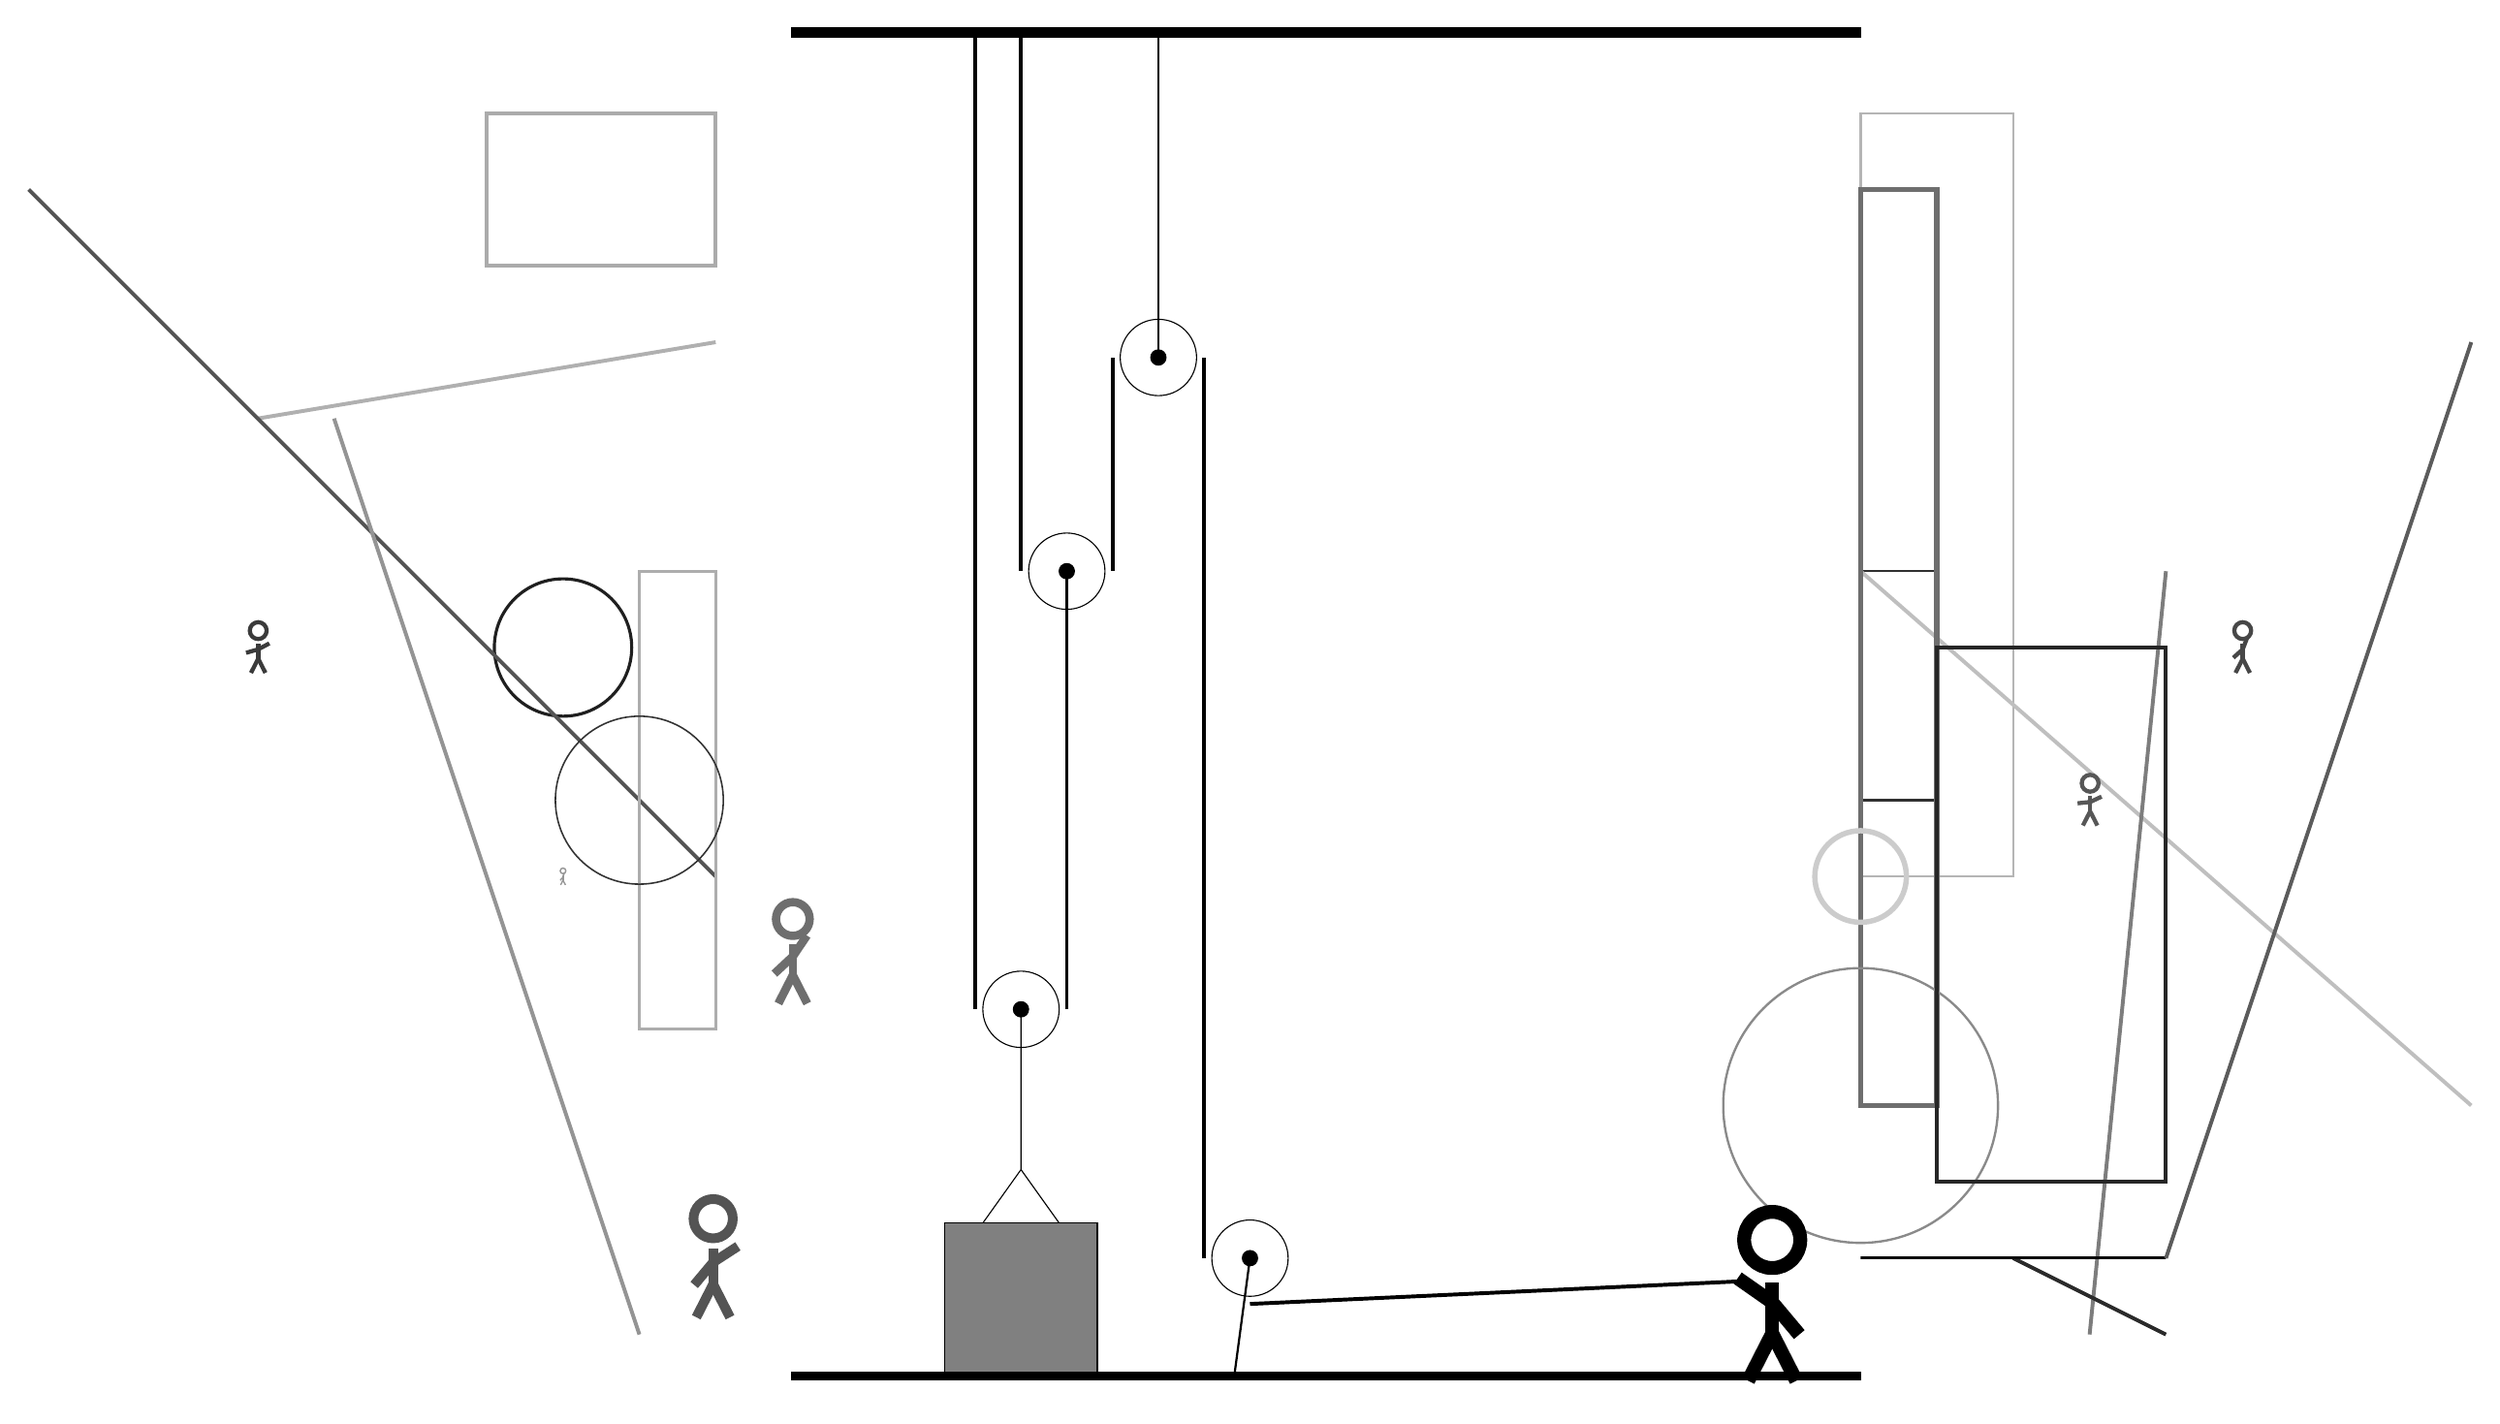
\begin{tikzpicture}
			%%%%% START %%%%%
			
			\draw[fill=black] (-2, 14) rectangle (12, 14.125);
			
			\draw (1, 1.26) circle (0.5);
			\draw[fill=black] (1, 1.26) circle (0.1);
			
			\draw (1.6, 7.0) circle (0.5);
			\draw[fill=black] (1.6, 7.0) circle (0.1);
			
			\draw (2.8, 9.8) circle (0.5);
			\draw[fill=black] (2.8, 9.8) circle (0.1);
			\draw[thick] (2.8, 9.8) -- (2.8, 14);
			
			\draw (4.0, -2) circle (0.5);
			\draw[fill=black] (4.0, -2) circle (0.1);
			\draw[thick] (4.0, -2) -- (3.8, -3.5);
			
			\draw[line width=0.3mm, color=black!29] (14, 13) rectangle (12, 3);
			
			\draw[line width=0.3mm, color=black!81] (12, 4) rectangle (13, 7);
			\draw[line width=0.5mm, color=black!25](12, 7) -- (20, 0);
			\draw[line width=0.5mm, color=black!31](-3, 10) -- (-9, 9);
			\draw [line width=0.4mm, color=black!88](-5, 6) circle (0.9);
			\node[line width=0.6mm, color=black!57] at (-2, 2) {\Strichmaxerl[6][43][56]};
			\draw[line width=0.5mm, color=black!51](15, -3) -- (16, 7);
			
			\draw[line width=0.5mm, color=black!67](-3, 3) -- (-12, 12);
			\draw[line width=0.5mm, color=black!83](14, -2) -- (16, -3);
			\node[line width=0.6mm, color=black!67] at (-3, -2) {\Strichmaxerl[7][50][33]};
			\draw[line width=0.4mm, color=black!32] (-3, 7) rectangle (-4, 1);
			\node[line width=0.7mm, color=black!66] at (15, 4) {\Strichmaxerl[3][6][25]};
			\draw[line width=0.4mm, color=black!96] (12, -2) rectangle (16, -2);
			
			\draw[line width=0.5mm, color=black!64](16, -2) -- (20, 10);
			\draw[line width=0.7mm, color=black!57] (13, 0) rectangle (12, 12);
			\node[line width=0.6mm, color=black!41] at (-5, 3) {\Strichmaxerl[1][49][74]};
			\draw [line width=0.2mm, color=black!80](-4, 4) circle (1.1);
			\draw [line width=0.3mm, color=black!46](12, 0) circle (1.8);
			\draw [line width=0.7mm, color=black!20](12, 3) circle (0.6);
			\node[line width=0.2mm, color=black!77] at (-9, 6) {\Strichmaxerl[3][16][28]};
			\draw[line width=0.5mm, color=black!33] (-3, 13) rectangle (-6, 11);
			\node[line width=0.2mm, color=black!72] at (17, 6) {\Strichmaxerl[3][42][69]};
			\draw[line width=0.5mm, color=black!85] (13, -1) rectangle (16, 6);
			\draw[line width=0.5mm, color=black!42](-4, -3) -- (-8, 9);
			
			\draw (1, 1.26) -- (1, -0.84) -- (0.5, -1.54) -- (1.5, -1.54) -- (1, -0.84);
			\draw[fill=black!50] (0, -1.54) rectangle (2, -3.54);
			\draw[line width=0.5mm] (0.4, 14) -- (0.4, 1.26);
			\centerarc[line width=0.5mm](1, 1.26)(180:360:0.6);
			\draw[line width=0.5mm](1.6, 1.26) -- (1.6, 7.0);
			\draw[line width=0.5mm] (1.0, 14) -- (1.0, 7.0);
			\centerarc[line width=0.5mm](1.6, 7.0)(180:360:0.6);
			\draw[line width=0.5mm](2.2, 7.0) -- (2.2, 9.8);
			\centerarc[line width=0.5mm](2.8, 9.8)(0:180:0.6);
			\draw[line width=0.5mm] (3.4, 9.8) -- (3.4, -2);
			\centerarc[line width=0.5mm](4.0, -2)(0:90:-0.6);
			\draw[line width=0.5mm](4.0, -2.6) -- (10.5, -2.3);
			
			\node at (10.8, -2.5) {\Strichmaxerl[10][-35][-50]};
			
			\draw[fill=black] (-2, -3.5) rectangle (12, -3.6);
			
			%%%%% END %%%%%
		\end{tikzpicture}
	\end{figure}	
\end{document}